\documentclass{acm_proc_article-sp-br}
%\documentclass{sig-alternate}


\usepackage{xspace}
\usepackage{graphicx,url}
\usepackage[brazil]{babel}
\usepackage[latin1]{inputenc}
\usepackage{color,amsmath}


\newcommand{\rev}[1]{{\textbf{\color{green} #1}}}
\newcommand{\del}[1]{{\textbf{\color{red} #1}}}



\sloppy

\title{T�tulo}


\numberofauthors{4} % m�ximo 3 colunas com autores. Demais, ver instru��es no estilo.

\author{
\alignauthor Primeiro Autor\\
       \affaddr{Departamento}\\
       \affaddr{Institui��o}\\
       \affaddr{Caixa Postal 668}\\
       \affaddr{00000-000  Cidade-UF-Brasil}\\
       \email{email@...}\\
\alignauthor Segundo Autor\\
       \affaddr{Departamento}\\
       \affaddr{Institui��o}\\
       \affaddr{Caixa Postal 668}\\
       \affaddr{00000-000  Cidade-UF-Brasil}\\
       \email{email@...}
\alignauthor Terceiro Autor\\
       \affaddr{Departamento}\\
       \affaddr{Institui��o}\\
       \affaddr{Caixa Postal 668}\\
       \affaddr{00000-000  Cidade-UF-Brasil}\\
       \email{email@...}
}
\additionalauthors{Quarto Autor, Departamento, Institui��o. email@...}

\date{30 July 1999}




%******************************************************************************

\begin{document}

\maketitle

\begin{abstract}
Summary...
\end{abstract}

\begin{resumo}
Resumo...
\end{resumo}


\section{Introdu��o} \label{sec:introducao}
Introdu��o com exemplo de cita��o \cite{Pressman2000}.

A Figura \ref{fig} � um exemplo de inser��o de figura.

\begin{figure}[!ht]
  \centering
  %Using latex, figures must be in eps format
  %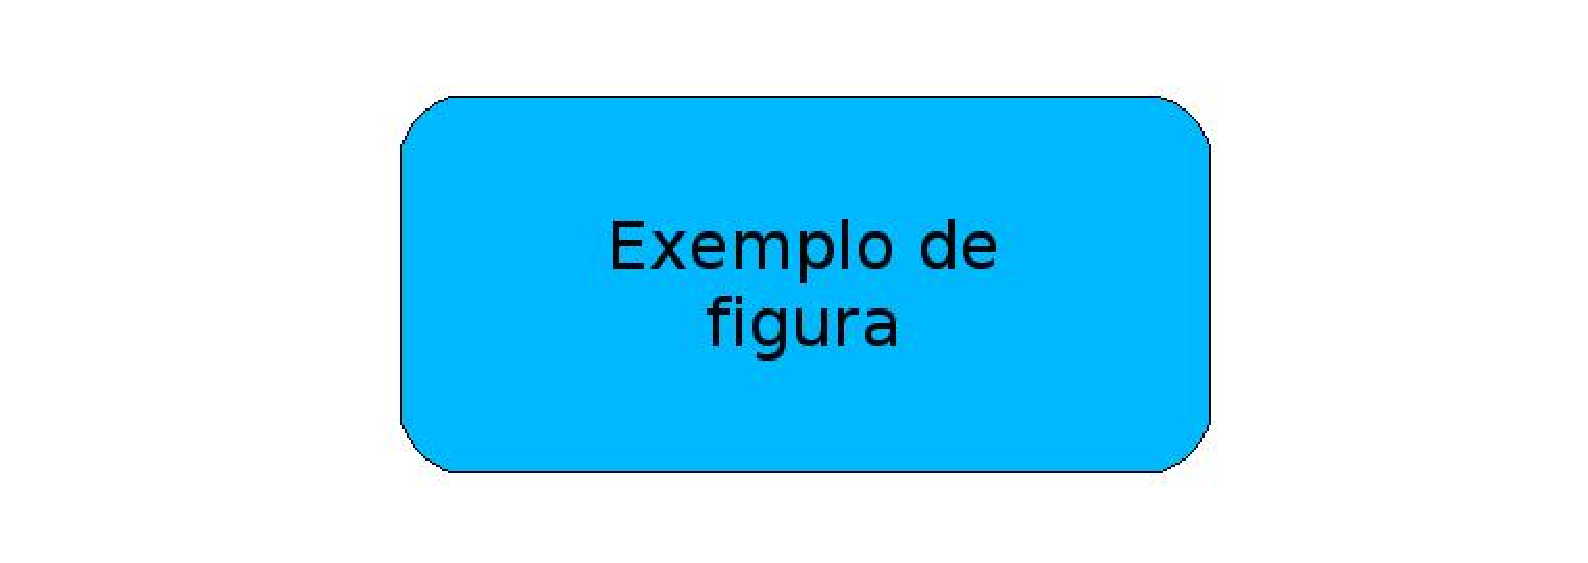
\includegraphics[width=.4\textwidth]{figura.eps}
  %Using pdflatex, figures can be in jpg
  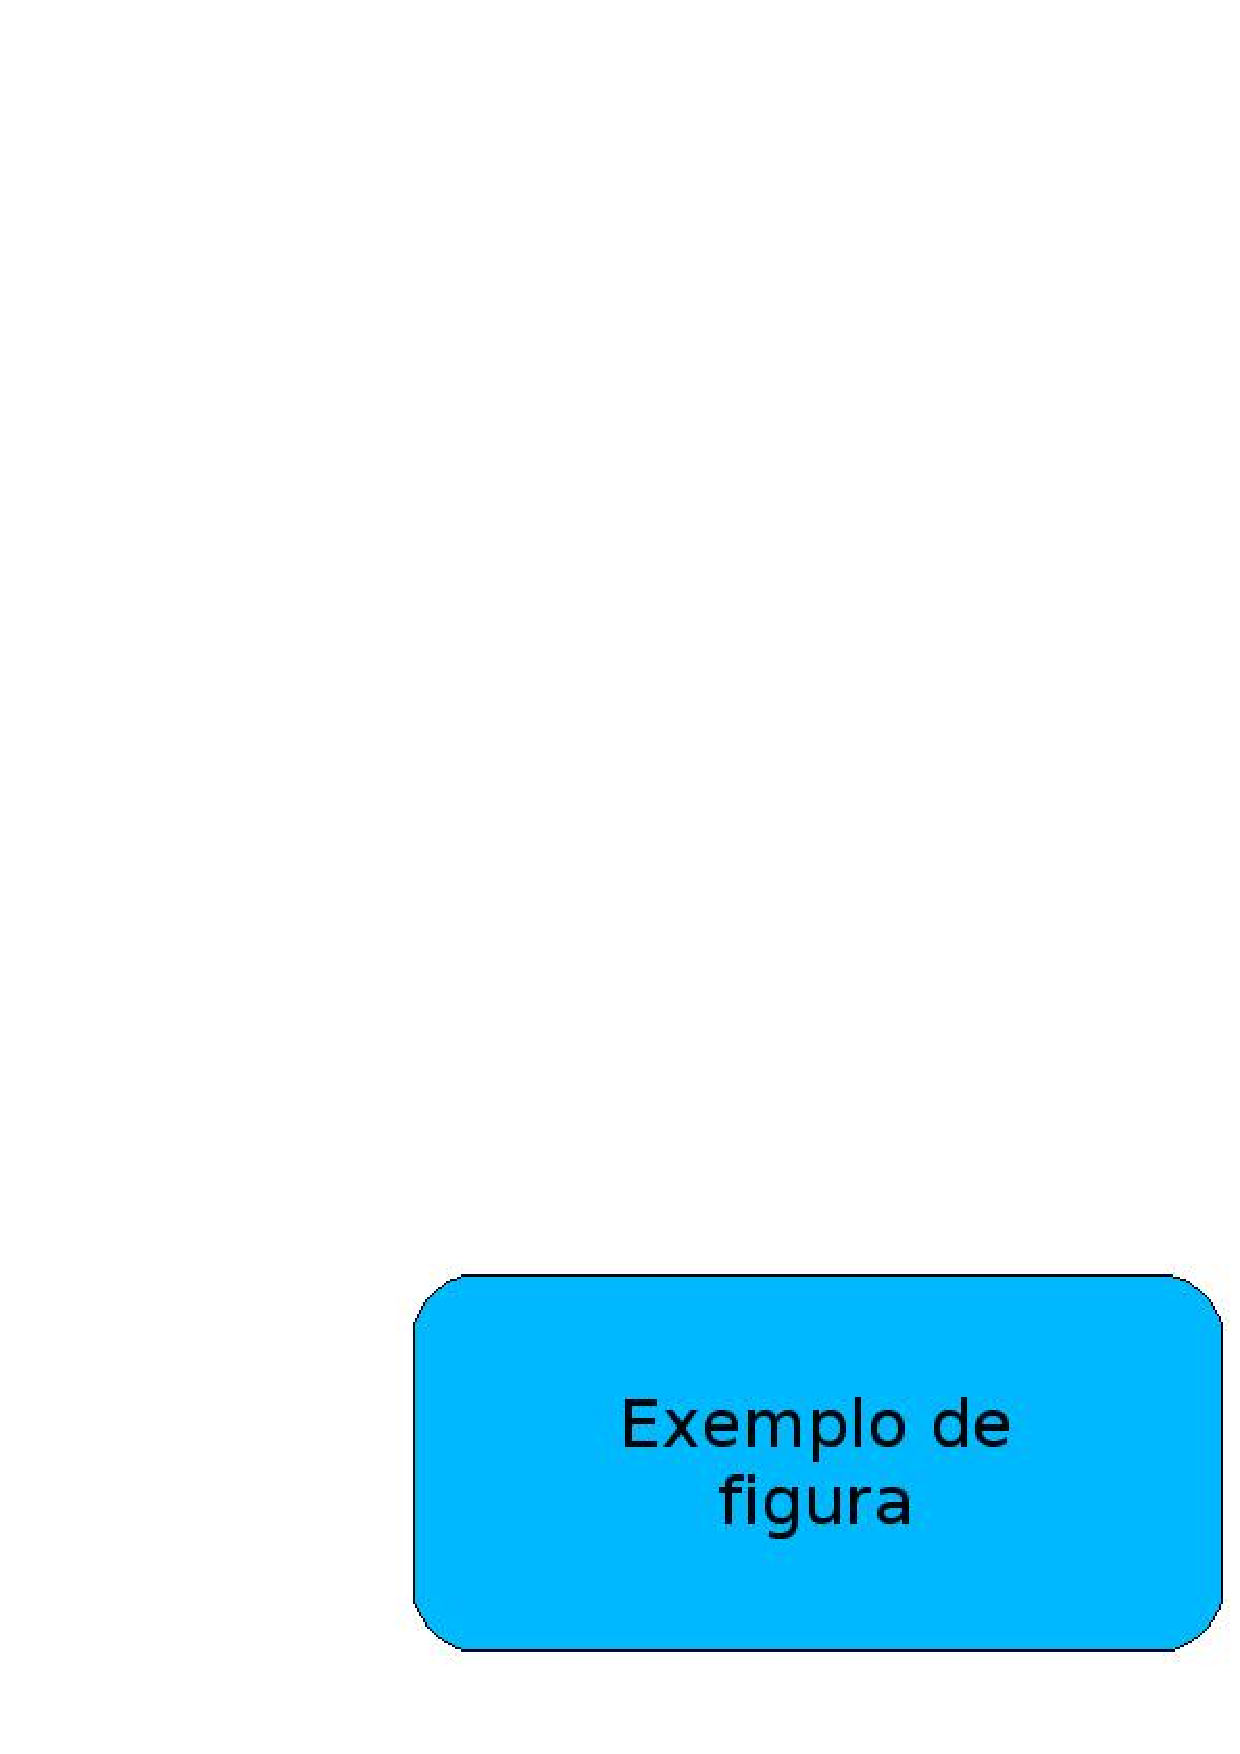
\includegraphics[width=.4\textwidth]{figura.jpg}
  \label{fig}
  \caption{Exemplo de inser��o de figura.}
\end{figure}


A Tabela \ref{tab} � um exemplo de tabela.

\begin{table}[!hb]
\centering
\label{tab}
\caption{Frequency of Special Characters}
\begin{tabular}{|c|c|l|} \hline
Non-English or Math&Frequency&Comments\\ \hline
\O & 1 in 1,000& For Swedish names\\ \hline
$\pi$ & 1 in 5& Common in math\\ \hline
\$ & 4 in 5 & Used in business\\ \hline
$\Psi^2_1$ & 1 in 40,000& Unexplained usage\\
\hline
\end{tabular}
\end{table}



\bibliographystyle{abbrv}
\bibliography{refs}

%\balancecolumns

\appendix
\section{T�tulo do ap�ndice}
Informa��s complementares...

\end{document}
